\documentclass{article}
\usepackage[utf8]{inputenc}
\usepackage[spanish]{babel}
\usepackage{listings}
\usepackage{graphicx}
\graphicspath{ {images/} }
\usepackage{cite}

\begin{document}

\begin{titlepage}
    \begin{center}
        \vspace*{1cm}
            
        \Huge
        \textbf{Trabajo de investigación}
            
        \vspace{0.5cm}
        \LARGE
        Nociones de la memoria de un computador
            
        \vspace{1.5cm}
            
        \textbf{Juliana Ruiz Sánchez}
            
        \vfill
            
        \vspace{0.8cm}
            
        \Large
        Despartamento de Ingeniería Electrónica y Telecomunicaciones\\
        Universidad de Antioquia\\
        Medellín\\
        Septiembre de 2020
            
    \end{center}
\end{titlepage}

\tableofcontents

\section{Sección introductoria}
Los computadores se han convertido en una parte fundamental de nuestra vida cotidiana, tanto para trabajar, estudiar o en los tiempos de ocio. La necesidad de tener un computador eficiente y veloz nos ha permitido avanzar ostensiblemente en materia tecnológica, lo que ha contribuido directamente a que estos aparatos sean más económicos para todos, sin que se deba sacrificar la calidad.


\section{Sección de contenido} \label{contenido}

\subsection{Definición}
La memoria de un computador es donde se almacena momentaneamente la información que necesitan los micorprocesadores para trabajar. Esta es indispensable para el buen funcionamiento del computador debido a que se mantiene comunicándose, en un ciclo constante, con el microprocesador.

\subsection{Tipos de memoria}

Existen diferentes tipos de memoria, diferenciándose en su funcionamiento y por consiguiente en su velocidad, entre más velocidad tiene menor es la capacidad de almacenamiento y más costosa.\newline

La más veloz es la memoria cache, se encuentra dentro del microprocesador y solo es utilizada por los programas más usados por el computador, se divide en L1, L2 y L3, siendo estas más veloces que la RAM; la L1 es la más rápida, la  L2 es más lenta que la anterior pero tiene mayor capacidad de almacenamiento, finalmente la L3 es la menos rápida pero es la que tiene mayor capacidad.
Figura (\ref{fig:Cache})\newline
\begin{figure}[h]
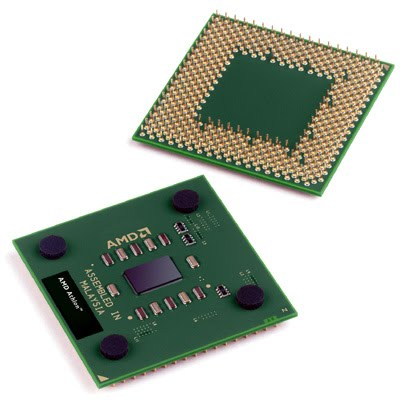
\includegraphics[width=3cm]{Cache.jpg}
\centering
\caption{Microprocesador, lugar donde se encuentra la memoria cache\cite{cache}}
\label{fig:Cache}
\end{figure}\newline
\newpage
La RAM(Random Access Memory), es del tipo DRAM(Dynamic Random Access Memory), esta almacena temporalmente bits (0 y 1) en otras palabras, datos. Está compuesta por celdas, en cada una de estas hay un capacitor y un transistor. Este tipo de memoria al solo contener uno de estos en cada celda es más económico, pero a su vez no es tan rápido como el microprocesador, demorándose al procesar la información y haciendo esperar a este.
Figura (\ref{fig:RAM})
\begin{figure}[h]
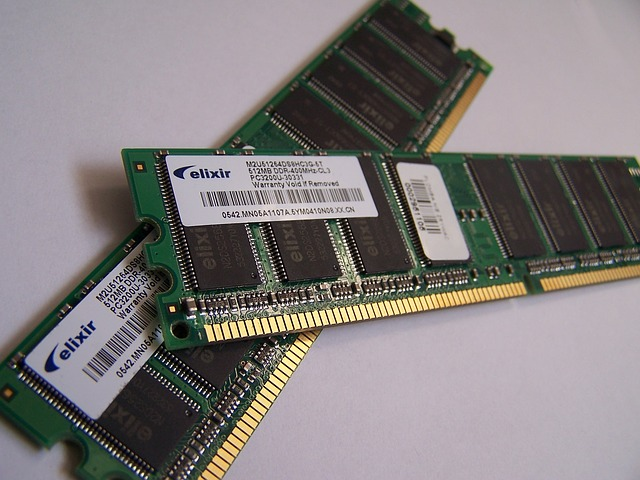
\includegraphics[width=4cm]{RAM.jpg}
\centering
\caption{Memoria RAM\cite{RAM}}
\label{fig:RAM}
\end{figure}\newline

La memoria virtual es una porción del disco duro que se dedica a contener temporalmente las partes y datos de ejecución menos utilizados, para siempre tenerlos a la mano.
Figura (\ref{fig:virtual})
\begin{figure}[h]
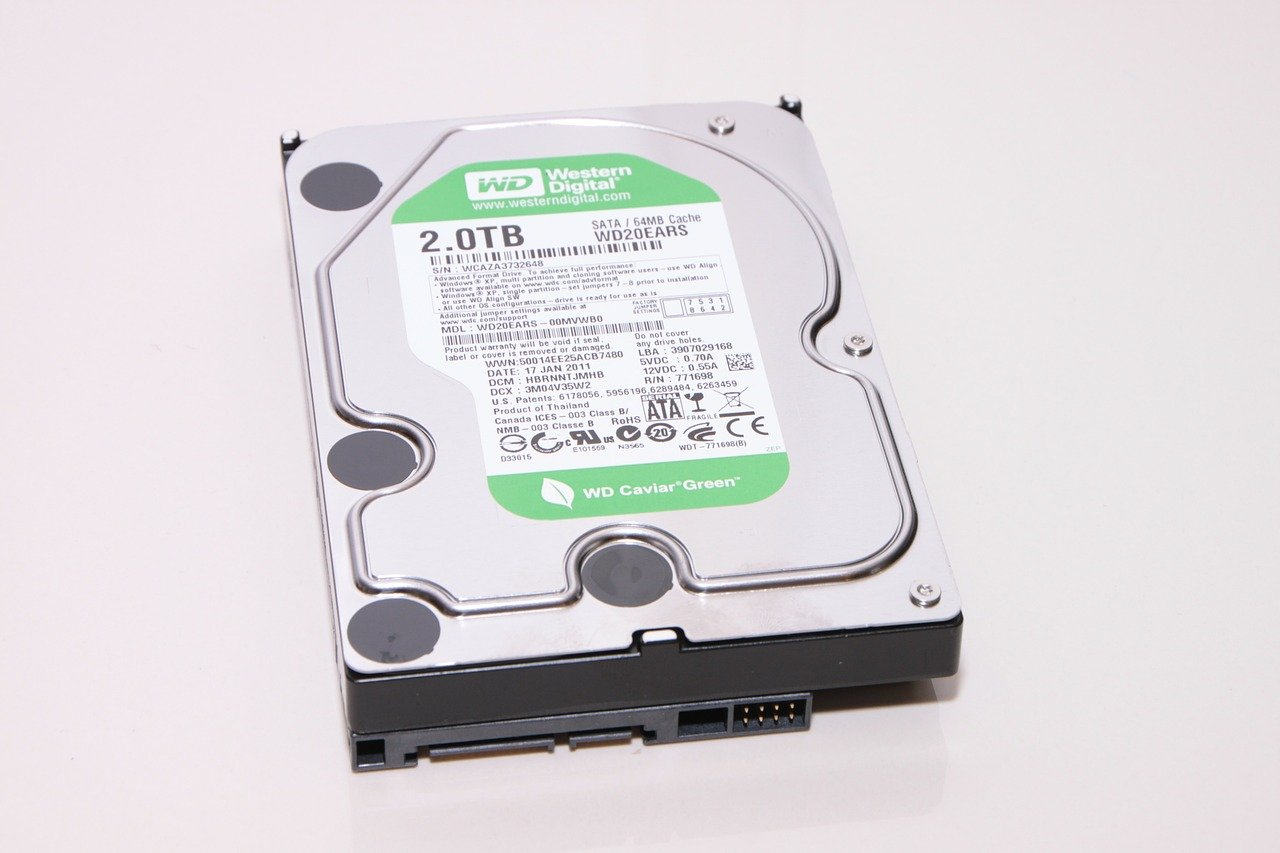
\includegraphics[width=4cm]{virtual.jpg}
\centering
\caption{Disco duro, lugar donde se encuentra la memoria virtual\cite{virtual}}
\label{fig:virtual}
\end{figure}\newline

El disco duro es la unidad de almacenamiento, en donde se guardan todos los datos y programas, debido a que este no borra los datos cada que el computador se apaga, como sucede con la memoria RAM. Es el menos veloz de todos, pero el que mayor capacidad de almacenamiento tiene gracias a su asequible precio (llega hasta las TB o TeraByte). Actualmente puede ser HDD(Hard Drive Disk) o SSD(Solid-State Drive); el HDD es el más utilizado debido a que es el más económico y tiene una gran capacidad de almacenamiento, se compone de placas de metal que giran constantemente y de un componente en forma de aguja el cual busca la posición de la infomación que se necesita (Figura (\ref{fig:HDD})). El SSD no gira constantemente sino que almacena la información por bloques, siendo así más rápido y duradero que el HDD pero, debido a su complicado funcionamiento,su costo es más elevado.
Figura (\ref{fig:SSD})\newline

\begin{figure}[h]
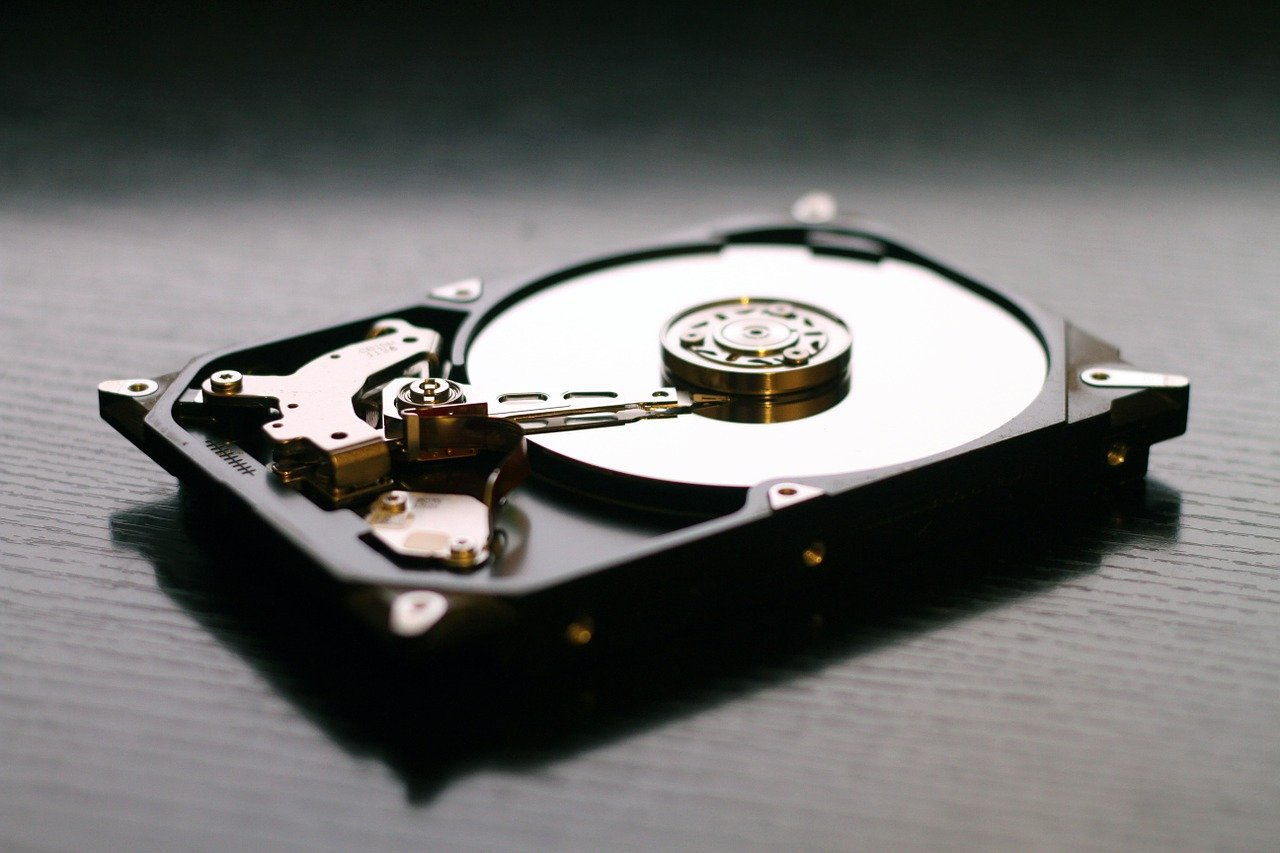
\includegraphics[width=4cm]{HDD.jpg}
\centering
\caption{Disco duro o HDD\cite{HDD}}
\label{fig:HDD}
\end{figure}

\begin{figure}[h]
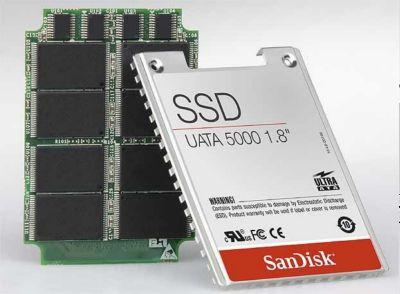
\includegraphics[width=4cm]{SSD.jpg}
\centering
\caption{Disco de estado sólido o SSD\cite{SSD}}
\label{fig:SSD}
\end{figure}

\subsection{Gestión de la memoria}
La memoria tiene un papel muy importante en el buen funcionamiento del computador, debido a que sin una de estas no se tendría la velocidad o capacidad requerida. Desde que se prende el computador hasta que se apaga, la memoria siempre está presente en todas las acciones que hacemos. Al prender un computador el microprocesador aún no ha comenzado a recibir órdenes, la primer órden se la da la memoria ROM(Read Only Memory), la cual le ordena que chequee los componentes más importantes del sistema, una vez comprueba que tienen buen funcionamiento carga la BIOS(Basic Input Output System), encargada de mostrar los dispositivos de almacenamiento, el disco de arranque y dispositivos externos; al darle esta información al microprocesador, este ya puede cargar el sistema operativo, ubicado en el disco duro, a la RAM, el cual permanecerá todo el timpo en esta y nos permitirá manejar el computador. Cada que abramos un programa o archivo en el computador, el microprocesador hace una copia en la RAM o, si es muy utilizado, en la memoria cache gracias a que esta es mucho más rápida que el disco duro. El microprocesador recibe órdenes, toma los datos, los procesa y los coloca, modificados, en el disco duro, haciendo este ciclo millones de veces por segundo

\subsection{Rapidez de una memoria}
La rapidez de la memoria es una de las cosas más importantes para tener un computador eficiente, tiene que ver con sus componentes y la forma de funcionar, por eso entre más eficiente sea la memoria, más cara y más complejo es su funcionamiento. La forma de saber el rendimiento de un computador es por medio de la latencia, esta sirve para medir la cantidad de tiempo que tarda la memoria en obterner los bits de información. Un ejemplo de esto es la memoria cache, compuesta de celdas en donde se almacena bits por medio de cuatro o seis transistores y algunos circuitos, al tener una gran cantidad de circuitos hay menos celdas, por lo que su capacidad es menor; por el contrario la memoria DRAM almacena en sus celdas bits por medio de un capacitor y un transistor, teniendo mayor cantidad de celdas (mayor espacio de almacenamiento) al no necesitar tantos componentes es más económica pero no tan rápida como la cache.

Documento basado en \cite{taller}

\section{Conclusión} \label{conclulsion}
La memoria es una parte indispensable del computador, sin ella no habría un correcto funcionamiento de este debido a que es la encargada de recibir las ordenes que recibe el microprocesador y de almacenar temporalmente copias de programas o archivos del disco duro para mayor eficiencia y velocidad del computador. Sin su correcto funcionamiento, el microprocesador se quedaría sin tareas que cumplir.

\bibliographystyle{IEEEtran}
\bibliography{references}

\end{document}
